\documentclass[]{article}
\usepackage{lmodern}
\usepackage{amssymb,amsmath}
\usepackage{ifxetex,ifluatex}
\usepackage{fixltx2e} % provides \textsubscript
\ifnum 0\ifxetex 1\fi\ifluatex 1\fi=0 % if pdftex
  \usepackage[T1]{fontenc}
  \usepackage[utf8]{inputenc}
\else % if luatex or xelatex
  \ifxetex
    \usepackage{mathspec}
  \else
    \usepackage{fontspec}
  \fi
  \defaultfontfeatures{Ligatures=TeX,Scale=MatchLowercase}
\fi
% use upquote if available, for straight quotes in verbatim environments
\IfFileExists{upquote.sty}{\usepackage{upquote}}{}
% use microtype if available
\IfFileExists{microtype.sty}{%
\usepackage{microtype}
\UseMicrotypeSet[protrusion]{basicmath} % disable protrusion for tt fonts
}{}
\usepackage[margin=1in]{geometry}
\usepackage{hyperref}
\hypersetup{unicode=true,
            pdftitle={Scientific papers on `Taper functions'},
            pdfauthor={prof. Roberto Scotti},
            pdfborder={0 0 0},
            breaklinks=true}
\urlstyle{same}  % don't use monospace font for urls
\usepackage{natbib}
\bibliographystyle{plainnat}
\usepackage{longtable,booktabs}
\usepackage{graphicx,grffile}
\makeatletter
\def\maxwidth{\ifdim\Gin@nat@width>\linewidth\linewidth\else\Gin@nat@width\fi}
\def\maxheight{\ifdim\Gin@nat@height>\textheight\textheight\else\Gin@nat@height\fi}
\makeatother
% Scale images if necessary, so that they will not overflow the page
% margins by default, and it is still possible to overwrite the defaults
% using explicit options in \includegraphics[width, height, ...]{}
\setkeys{Gin}{width=\maxwidth,height=\maxheight,keepaspectratio}
\IfFileExists{parskip.sty}{%
\usepackage{parskip}
}{% else
\setlength{\parindent}{0pt}
\setlength{\parskip}{6pt plus 2pt minus 1pt}
}
\setlength{\emergencystretch}{3em}  % prevent overfull lines
\providecommand{\tightlist}{%
  \setlength{\itemsep}{0pt}\setlength{\parskip}{0pt}}
\setcounter{secnumdepth}{0}
% Redefines (sub)paragraphs to behave more like sections
\ifx\paragraph\undefined\else
\let\oldparagraph\paragraph
\renewcommand{\paragraph}[1]{\oldparagraph{#1}\mbox{}}
\fi
\ifx\subparagraph\undefined\else
\let\oldsubparagraph\subparagraph
\renewcommand{\subparagraph}[1]{\oldsubparagraph{#1}\mbox{}}
\fi

%%% Use protect on footnotes to avoid problems with footnotes in titles
\let\rmarkdownfootnote\footnote%
\def\footnote{\protect\rmarkdownfootnote}

%%% Change title format to be more compact
\usepackage{titling}

% Create subtitle command for use in maketitle
\newcommand{\subtitle}[1]{
  \posttitle{
    \begin{center}\large#1\end{center}
    }
}

\setlength{\droptitle}{-2em}

  \title{Scientific papers on `Taper functions'}
    \pretitle{\vspace{\droptitle}\centering\huge}
  \posttitle{\par}
    \author{prof. Roberto Scotti \footnote{NuoroForestrySchool -
  \href{mailto:scotti@uniss.it}{\nolinkurl{scotti@uniss.it}}}}
    \preauthor{\centering\large\emph}
  \postauthor{\par}
      \predate{\centering\large\emph}
  \postdate{\par}
    \date{25 ago 2018}

\usepackage[labelformat=empty]{caption}

\begin{document}
\maketitle

\hypertarget{introduction}{%
\section{Introduction}\label{introduction}}

\hypertarget{forest-inventory-course---first-results-of-the-collective-assignement}{%
\subsection{2018 Forest Inventory course - First results of the
collective
assignement}\label{forest-inventory-course---first-results-of-the-collective-assignement}}

Students, as homework, were asked to search for scientific papers
presenting `taper functions' and to compile a collective Rmarkdown
document shared using GIT.\\
Rearranging their work, this document lists their findings.

\hypertarget{analysed-articles}{%
\section{Analysed articles}\label{analysed-articles}}

\#\#Article ID 1 : \emph{(Scolforo, McTague, Raimundo, et al., 2018)}
\textbf{Comparison of taper functions applied to eucalypts of varying
genetics in \{Brazil\}: application and evaluation of the penalized
mixed spline approach}

\begin{longtable}[]{@{}ll@{}}
\toprule
\endhead
\begin{minipage}[t]{0.21\columnwidth}\raggedright
Student\strut
\end{minipage} & \begin{minipage}[t]{0.73\columnwidth}\raggedright
Angelo Manca\strut
\end{minipage}\tabularnewline
\begin{minipage}[t]{0.21\columnwidth}\raggedright
Title.student\strut
\end{minipage} & \begin{minipage}[t]{0.73\columnwidth}\raggedright
Comparison of taper functions applied to eucalypts of varying genetics
in Brazil: Application and evaluation of the penalized mixed spline
approach\strut
\end{minipage}\tabularnewline
\begin{minipage}[t]{0.21\columnwidth}\raggedright
Authors.student\strut
\end{minipage} & \begin{minipage}[t]{0.73\columnwidth}\raggedright
Scolforo, H.F., McTague, J.P., Raimundo, M.R., Weiskittel, A., Carrero,
O., Scolforo, J.R.S.\strut
\end{minipage}\tabularnewline
\begin{minipage}[t]{0.21\columnwidth}\raggedright
Year.student\strut
\end{minipage} & \begin{minipage}[t]{0.73\columnwidth}\raggedright
2017\strut
\end{minipage}\tabularnewline
\begin{minipage}[t]{0.21\columnwidth}\raggedright
Species\strut
\end{minipage} & \begin{minipage}[t]{0.73\columnwidth}\raggedright
Eucalypts\strut
\end{minipage}\tabularnewline
\begin{minipage}[t]{0.21\columnwidth}\raggedright
Base.URL\strut
\end{minipage} & \begin{minipage}[t]{0.73\columnwidth}\raggedright
\url{http://www.nrcresearchpress.com/doi/10.1139/cjfr-2017-0366\#.W2Sb6Lhx02w}\strut
\end{minipage}\tabularnewline
\begin{minipage}[t]{0.21\columnwidth}\raggedright
Paper.local.file\strut
\end{minipage} & \begin{minipage}[t]{0.73\columnwidth}\raggedright
NA\strut
\end{minipage}\tabularnewline
\begin{minipage}[t]{0.21\columnwidth}\raggedright
Equations\strut
\end{minipage} & \begin{minipage}[t]{0.73\columnwidth}\raggedright
NA\strut
\end{minipage}\tabularnewline
\bottomrule
\end{longtable}

\#\#Article ID 2 : \emph{(Warner, Jamroenprucksa, and Puangchit, 2016)}
\textbf{Development and evaluation of teak (\{Tectona\} grandis
\{L\}.f.) taper equations in northern \{Thailand\}}

\begin{longtable}[]{@{}ll@{}}
\toprule
\endhead
\begin{minipage}[t]{0.21\columnwidth}\raggedright
Student\strut
\end{minipage} & \begin{minipage}[t]{0.73\columnwidth}\raggedright
Angelo Manca\strut
\end{minipage}\tabularnewline
\begin{minipage}[t]{0.21\columnwidth}\raggedright
Title.student\strut
\end{minipage} & \begin{minipage}[t]{0.73\columnwidth}\raggedright
Development and evaluation of teak (Tectona grandis L.f.) taper
equations in northern Thailand,\strut
\end{minipage}\tabularnewline
\begin{minipage}[t]{0.21\columnwidth}\raggedright
Authors.student\strut
\end{minipage} & \begin{minipage}[t]{0.73\columnwidth}\raggedright
Andrew J. Warner, Monton Jamroenprucksa, Ladawan Puangchit,\strut
\end{minipage}\tabularnewline
\begin{minipage}[t]{0.21\columnwidth}\raggedright
Year.student\strut
\end{minipage} & \begin{minipage}[t]{0.73\columnwidth}\raggedright
2016\strut
\end{minipage}\tabularnewline
\begin{minipage}[t]{0.21\columnwidth}\raggedright
Species\strut
\end{minipage} & \begin{minipage}[t]{0.73\columnwidth}\raggedright
Tectona grandis L.f.\strut
\end{minipage}\tabularnewline
\begin{minipage}[t]{0.21\columnwidth}\raggedright
Base.URL\strut
\end{minipage} & \begin{minipage}[t]{0.73\columnwidth}\raggedright
\url{https://www.sciencedirect.com/science/article/pii/S2452316X16302459?via\%3Dihub}\strut
\end{minipage}\tabularnewline
\begin{minipage}[t]{0.21\columnwidth}\raggedright
Paper.local.file\strut
\end{minipage} & \begin{minipage}[t]{0.73\columnwidth}\raggedright
1-s2.0-S2452316X16302459-main.pdf\strut
\end{minipage}\tabularnewline
\begin{minipage}[t]{0.21\columnwidth}\raggedright
Equations\strut
\end{minipage} & \begin{minipage}[t]{0.73\columnwidth}\raggedright
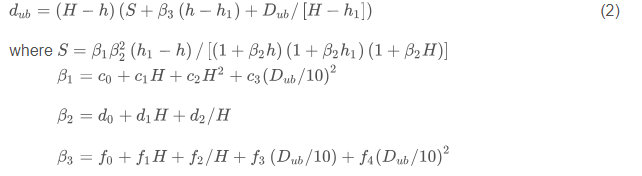
\includegraphics{Equations/2016WarnerEtAl.png}\strut
\end{minipage}\tabularnewline
\bottomrule
\end{longtable}

\#\#Article ID 3 : \emph{(Tang, Pérez-Cruzado, Fehrmann, et al., 2016)}
\textbf{Development of a \{Compatible\} \{Taper\} \{Function\} and
\{Stand\}-\{Level\} \{Merchantable\} \{Volume\} \{Model\} for
\{Chinese\} \{Fir\} \{Plantations\}}

\begin{longtable}[]{@{}ll@{}}
\toprule
\endhead
\begin{minipage}[t]{0.21\columnwidth}\raggedright
Student\strut
\end{minipage} & \begin{minipage}[t]{0.73\columnwidth}\raggedright
Angelo Manca\strut
\end{minipage}\tabularnewline
\begin{minipage}[t]{0.21\columnwidth}\raggedright
Title.student\strut
\end{minipage} & \begin{minipage}[t]{0.73\columnwidth}\raggedright
Development of a Compatible Taper Function and Stand-Level Merchantable
Volume Model for Chinese Fir Plantations\strut
\end{minipage}\tabularnewline
\begin{minipage}[t]{0.21\columnwidth}\raggedright
Authors.student\strut
\end{minipage} & \begin{minipage}[t]{0.73\columnwidth}\raggedright
Xiaolu Tang,César Pérez-Cruzado,Lutz Fehrmann,Juan Gabriel
Álvarez-González,Yuanchang Lu,and Christoph Kleinn,\strut
\end{minipage}\tabularnewline
\begin{minipage}[t]{0.21\columnwidth}\raggedright
Year.student\strut
\end{minipage} & \begin{minipage}[t]{0.73\columnwidth}\raggedright
2016\strut
\end{minipage}\tabularnewline
\begin{minipage}[t]{0.21\columnwidth}\raggedright
Species\strut
\end{minipage} & \begin{minipage}[t]{0.73\columnwidth}\raggedright
Cunninghamia lanceolata {[}Lamb.{]} Hook\strut
\end{minipage}\tabularnewline
\begin{minipage}[t]{0.21\columnwidth}\raggedright
Base.URL\strut
\end{minipage} & \begin{minipage}[t]{0.73\columnwidth}\raggedright
\url{https://www.ncbi.nlm.nih.gov/pubmed/26799399}\strut
\end{minipage}\tabularnewline
\begin{minipage}[t]{0.21\columnwidth}\raggedright
Paper.local.file\strut
\end{minipage} & \begin{minipage}[t]{0.73\columnwidth}\raggedright
pone.0147610.pdf\strut
\end{minipage}\tabularnewline
\begin{minipage}[t]{0.21\columnwidth}\raggedright
Equations\strut
\end{minipage} & \begin{minipage}[t]{0.73\columnwidth}\raggedright
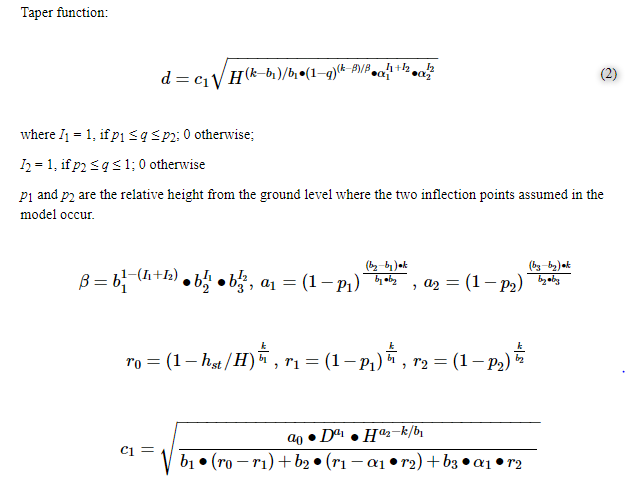
\includegraphics{Equations/2016TangEtAl.png}\strut
\end{minipage}\tabularnewline
\bottomrule
\end{longtable}

\#\#Article ID 4 : \emph{(Corral-Rivas, Vega-Nieva,
Rodríguez-Soalleiro, et al., 2017)} \textbf{Compatible \{System\} for
\{Predicting\} \{Total\} and \{Merchantable\} \{Stem\} \{Volume\} over
and under \{Bark\}, \{Branch\} \{Volume\} and \{Whole\}-\{Tree\}
\{Volume\} of \{Pine\} \{Species\}}

\begin{longtable}[]{@{}ll@{}}
\toprule
\endhead
\begin{minipage}[t]{0.21\columnwidth}\raggedright
Student\strut
\end{minipage} & \begin{minipage}[t]{0.73\columnwidth}\raggedright
Maria Chiara Ruggiu\strut
\end{minipage}\tabularnewline
\begin{minipage}[t]{0.21\columnwidth}\raggedright
Title.student\strut
\end{minipage} & \begin{minipage}[t]{0.73\columnwidth}\raggedright
Compatible System for Predicting Total and Merchantable Stem Volume over
and under Bark, Branch Volume and Whole-Tree Volume of Pine
Species"\strut
\end{minipage}\tabularnewline
\begin{minipage}[t]{0.21\columnwidth}\raggedright
Authors.student\strut
\end{minipage} & \begin{minipage}[t]{0.73\columnwidth}\raggedright
José Javier Corral-Rivas, Daniel Jose Vega-Nieva, Roque
Rodríguez-Soalleiro, Carlos Antonio López-Sánchez, Christian Wehenkel,
Benedicto Vargas-Larreta, Juan Gabriel Álvarez-González and Ana Daría
Ruiz-González.\strut
\end{minipage}\tabularnewline
\begin{minipage}[t]{0.21\columnwidth}\raggedright
Year.student\strut
\end{minipage} & \begin{minipage}[t]{0.73\columnwidth}\raggedright
2017\strut
\end{minipage}\tabularnewline
\begin{minipage}[t]{0.21\columnwidth}\raggedright
Species\strut
\end{minipage} & \begin{minipage}[t]{0.73\columnwidth}\raggedright
Pinus cooperi, Pinus durangensis\strut
\end{minipage}\tabularnewline
\begin{minipage}[t]{0.21\columnwidth}\raggedright
Base.URL\strut
\end{minipage} & \begin{minipage}[t]{0.73\columnwidth}\raggedright
\url{http://www.mdpi.com/1999-4907/8/11/417}\strut
\end{minipage}\tabularnewline
\begin{minipage}[t]{0.21\columnwidth}\raggedright
Paper.local.file\strut
\end{minipage} & \begin{minipage}[t]{0.73\columnwidth}\raggedright
forests-08-00417-v2.pdf\strut
\end{minipage}\tabularnewline
\begin{minipage}[t]{0.21\columnwidth}\raggedright
Equations\strut
\end{minipage} & \begin{minipage}[t]{0.73\columnwidth}\raggedright
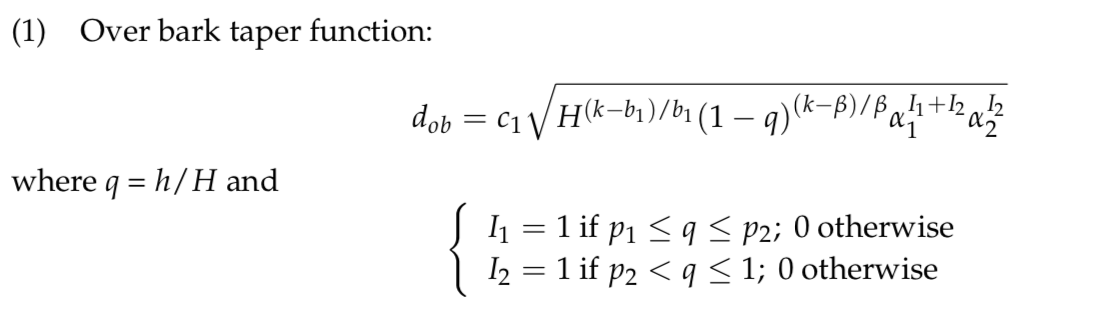
\includegraphics{Equations/2017Corral-RivasEtAlOb.png}\strut
\end{minipage}\tabularnewline
\begin{minipage}[t]{0.21\columnwidth}\raggedright
Equations\strut
\end{minipage} & \begin{minipage}[t]{0.73\columnwidth}\raggedright
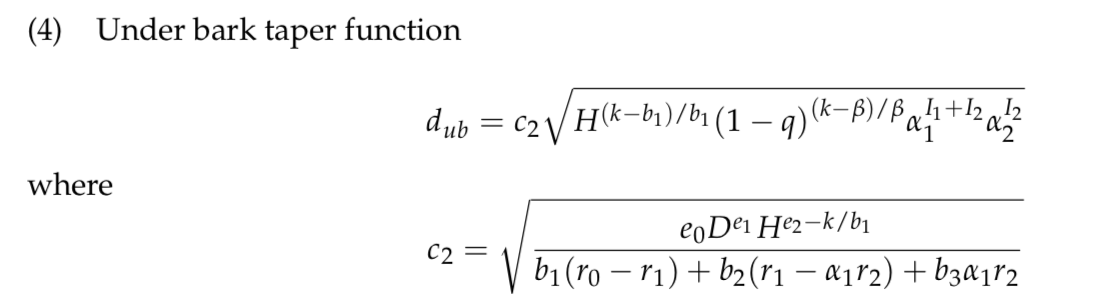
\includegraphics{Equations/2017Corral-RivasEtAlUb.png}\strut
\end{minipage}\tabularnewline
\bottomrule
\end{longtable}

\#\#Article ID 5 : \emph{(Sun, Liang, Liang, et al., 2016)}
\textbf{Deriving \{Merchantable\} \{Volume\} in \{Poplar\} through a
\{Localized\} \{Tapering\} \{Function\} from \{Non\}-\{Destructive\}
\{Terrestrial\} \{Laser\} \{Scanning\}}

\begin{longtable}[]{@{}ll@{}}
\toprule
\endhead
\begin{minipage}[t]{0.21\columnwidth}\raggedright
Student\strut
\end{minipage} & \begin{minipage}[t]{0.73\columnwidth}\raggedright
Matteo Piccolo\strut
\end{minipage}\tabularnewline
\begin{minipage}[t]{0.21\columnwidth}\raggedright
Title.student\strut
\end{minipage} & \begin{minipage}[t]{0.73\columnwidth}\raggedright
Deriving Merchantable Volume in Poplar through a Localized Tapering
Function from Non-Destructive Terrestrial Laser Scanning\strut
\end{minipage}\tabularnewline
\begin{minipage}[t]{0.21\columnwidth}\raggedright
Authors.student\strut
\end{minipage} & \begin{minipage}[t]{0.73\columnwidth}\raggedright
Yuan Sun, Xinlian Liang, Ziyu Liang, Clive Welham and Weizheng Li\strut
\end{minipage}\tabularnewline
\begin{minipage}[t]{0.21\columnwidth}\raggedright
Year.student\strut
\end{minipage} & \begin{minipage}[t]{0.73\columnwidth}\raggedright
2016\strut
\end{minipage}\tabularnewline
\begin{minipage}[t]{0.21\columnwidth}\raggedright
Species\strut
\end{minipage} & \begin{minipage}[t]{0.73\columnwidth}\raggedright
Populus × canadensis Moench cv.\strut
\end{minipage}\tabularnewline
\begin{minipage}[t]{0.21\columnwidth}\raggedright
Base.URL\strut
\end{minipage} & \begin{minipage}[t]{0.73\columnwidth}\raggedright
\url{http://www.mdpi.com/1999-4907/7/4/87/htm}\strut
\end{minipage}\tabularnewline
\begin{minipage}[t]{0.21\columnwidth}\raggedright
Paper.local.file\strut
\end{minipage} & \begin{minipage}[t]{0.73\columnwidth}\raggedright
forests-07-00087.pdf\strut
\end{minipage}\tabularnewline
\begin{minipage}[t]{0.21\columnwidth}\raggedright
Equations\strut
\end{minipage} & \begin{minipage}[t]{0.73\columnwidth}\raggedright
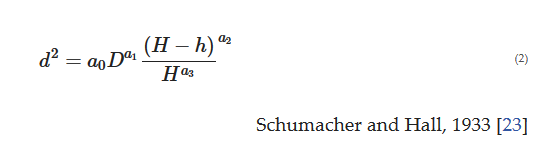
\includegraphics{Equations/2016Sunetal.png}\strut
\end{minipage}\tabularnewline
\bottomrule
\end{longtable}

\#\#Article ID 6 : \emph{(Martins, Debastiani, Pelissari, et al., 2017)}
\textbf{Estimativa do \{Afilamento\} do \{Fuste\} de \{Araucária\}
\{Utilizando\} \{Técnicas\} de \{Inteligência\} \{Artificial\}}

\begin{longtable}[]{@{}ll@{}}
\toprule
\endhead
\begin{minipage}[t]{0.21\columnwidth}\raggedright
Student\strut
\end{minipage} & \begin{minipage}[t]{0.73\columnwidth}\raggedright
Maria Chiara Ruggiu\strut
\end{minipage}\tabularnewline
\begin{minipage}[t]{0.21\columnwidth}\raggedright
Title.student\strut
\end{minipage} & \begin{minipage}[t]{0.73\columnwidth}\raggedright
Araucaria Stem Taper or Use of Artificial Intelligence Techniques\strut
\end{minipage}\tabularnewline
\begin{minipage}[t]{0.21\columnwidth}\raggedright
Authors.student\strut
\end{minipage} & \begin{minipage}[t]{0.73\columnwidth}\raggedright
Ana Paula Marques Martins, Aline Bernarda Debastiani, Allan Libanio
Pelissari, Sebastião do Amaral Machado, Carlos Roberto Sanquetta\strut
\end{minipage}\tabularnewline
\begin{minipage}[t]{0.21\columnwidth}\raggedright
Year.student\strut
\end{minipage} & \begin{minipage}[t]{0.73\columnwidth}\raggedright
2017\strut
\end{minipage}\tabularnewline
\begin{minipage}[t]{0.21\columnwidth}\raggedright
Species\strut
\end{minipage} & \begin{minipage}[t]{0.73\columnwidth}\raggedright
Araucaria angustifolia\strut
\end{minipage}\tabularnewline
\begin{minipage}[t]{0.21\columnwidth}\raggedright
Base.URL\strut
\end{minipage} & \begin{minipage}[t]{0.73\columnwidth}\raggedright
\url{http://www.scielo.br/scielo.php?script=sci_arttext\&pid=S2179-80872017000100152}\strut
\end{minipage}\tabularnewline
\begin{minipage}[t]{0.21\columnwidth}\raggedright
Paper.local.file\strut
\end{minipage} & \begin{minipage}[t]{0.73\columnwidth}\raggedright
2179-8087-floram-24-e20160234.pdf\strut
\end{minipage}\tabularnewline
\begin{minipage}[t]{0.21\columnwidth}\raggedright
Equations\strut
\end{minipage} & \begin{minipage}[t]{0.73\columnwidth}\raggedright
NA\strut
\end{minipage}\tabularnewline
\bottomrule
\end{longtable}

\#\#Article ID 7 : \emph{(Silva, Rodriguez, Caixeta Filho, et al.,
2006)} \textbf{Fitting a taper function to minimize the sum of absolute
deviations}

\begin{longtable}[]{@{}ll@{}}
\toprule
\endhead
\begin{minipage}[t]{0.21\columnwidth}\raggedright
Student\strut
\end{minipage} & \begin{minipage}[t]{0.73\columnwidth}\raggedright
Maria Chiara Ruggiu\strut
\end{minipage}\tabularnewline
\begin{minipage}[t]{0.21\columnwidth}\raggedright
Title.student\strut
\end{minipage} & \begin{minipage}[t]{0.73\columnwidth}\raggedright
Fitting a taper function to minimize the sum of absolute
deviations\strut
\end{minipage}\tabularnewline
\begin{minipage}[t]{0.21\columnwidth}\raggedright
Authors.student\strut
\end{minipage} & \begin{minipage}[t]{0.73\columnwidth}\raggedright
Lana Mirian Santos da Silva, Luiz Carlos Estraviz Rodriguez, José
Vicente Caixeta Filho; Simone Carolina Bauch\strut
\end{minipage}\tabularnewline
\begin{minipage}[t]{0.21\columnwidth}\raggedright
Year.student\strut
\end{minipage} & \begin{minipage}[t]{0.73\columnwidth}\raggedright
2006\strut
\end{minipage}\tabularnewline
\begin{minipage}[t]{0.21\columnwidth}\raggedright
Species\strut
\end{minipage} & \begin{minipage}[t]{0.73\columnwidth}\raggedright
Eucalyptus\strut
\end{minipage}\tabularnewline
\begin{minipage}[t]{0.21\columnwidth}\raggedright
Base.URL\strut
\end{minipage} & \begin{minipage}[t]{0.73\columnwidth}\raggedright
\url{http://www.scielo.br/scielo.php?script=sci_arttext\&pid=S0103-90162006000500007}\strut
\end{minipage}\tabularnewline
\begin{minipage}[t]{0.21\columnwidth}\raggedright
Paper.local.file\strut
\end{minipage} & \begin{minipage}[t]{0.73\columnwidth}\raggedright
31406.pdf\strut
\end{minipage}\tabularnewline
\begin{minipage}[t]{0.21\columnwidth}\raggedright
Equations\strut
\end{minipage} & \begin{minipage}[t]{0.73\columnwidth}\raggedright
NA\strut
\end{minipage}\tabularnewline
\bottomrule
\end{longtable}

\#\#Article ID 8 : \emph{(Arnoni Costa, Guimarães Finger, Schneider, et
al., 2016)} \textbf{\{FUNÇÃO\} \{DE\} \{AFILAMENTO\} \{E\}
\{SORTIMENTOS\} \{DE\} \{MADEIRA\} \{PARA\} \{Araucaria\} angustifolia}

\begin{longtable}[]{@{}ll@{}}
\toprule
\endhead
\begin{minipage}[t]{0.21\columnwidth}\raggedright
Student\strut
\end{minipage} & \begin{minipage}[t]{0.73\columnwidth}\raggedright
Maria Chiara Ruggiu\strut
\end{minipage}\tabularnewline
\begin{minipage}[t]{0.21\columnwidth}\raggedright
Title.student\strut
\end{minipage} & \begin{minipage}[t]{0.73\columnwidth}\raggedright
Taper function and timber assortments for Araucaria angustifolia\strut
\end{minipage}\tabularnewline
\begin{minipage}[t]{0.21\columnwidth}\raggedright
Authors.student\strut
\end{minipage} & \begin{minipage}[t]{0.73\columnwidth}\raggedright
Emanuel Arnoni Costa, César Augusto Guimarães Finger, Paulo Renato
Schneider, André Felipe Hess\strut
\end{minipage}\tabularnewline
\begin{minipage}[t]{0.21\columnwidth}\raggedright
Year.student\strut
\end{minipage} & \begin{minipage}[t]{0.73\columnwidth}\raggedright
2016\strut
\end{minipage}\tabularnewline
\begin{minipage}[t]{0.21\columnwidth}\raggedright
Species\strut
\end{minipage} & \begin{minipage}[t]{0.73\columnwidth}\raggedright
Araucaria angustifolia\strut
\end{minipage}\tabularnewline
\begin{minipage}[t]{0.21\columnwidth}\raggedright
Base.URL\strut
\end{minipage} & \begin{minipage}[t]{0.73\columnwidth}\raggedright
\url{http://www.redalyc.org/articulo.oa?id=53446151016}\strut
\end{minipage}\tabularnewline
\begin{minipage}[t]{0.21\columnwidth}\raggedright
Paper.local.file\strut
\end{minipage} & \begin{minipage}[t]{0.73\columnwidth}\raggedright
53446151016.pdf\strut
\end{minipage}\tabularnewline
\begin{minipage}[t]{0.21\columnwidth}\raggedright
Equations\strut
\end{minipage} & \begin{minipage}[t]{0.73\columnwidth}\raggedright
NA\strut
\end{minipage}\tabularnewline
\bottomrule
\end{longtable}

\#\#Article ID 9 : \emph{(Souza, Chassot, Finger, et al., 2008)}
\textbf{Modelos de afilamento para o sortimento do fuste de \{Pinus\}
taeda \{L\}}

\begin{longtable}[]{@{}ll@{}}
\toprule
\endhead
\begin{minipage}[t]{0.21\columnwidth}\raggedright
Student\strut
\end{minipage} & \begin{minipage}[t]{0.73\columnwidth}\raggedright
Matteo Piccolo\strut
\end{minipage}\tabularnewline
\begin{minipage}[t]{0.21\columnwidth}\raggedright
Title.student\strut
\end{minipage} & \begin{minipage}[t]{0.73\columnwidth}\raggedright
Taper function for assortment of Pinus taeda L. stem\strut
\end{minipage}\tabularnewline
\begin{minipage}[t]{0.21\columnwidth}\raggedright
Authors.student\strut
\end{minipage} & \begin{minipage}[t]{0.73\columnwidth}\raggedright
Carlos Alberto Martinelli de Souza, Tatiane Chassot, César Augusto
Guimarães Finger, Paulo Renato Schneider, Frederico Dimas Fleig\strut
\end{minipage}\tabularnewline
\begin{minipage}[t]{0.21\columnwidth}\raggedright
Year.student\strut
\end{minipage} & \begin{minipage}[t]{0.73\columnwidth}\raggedright
2008\strut
\end{minipage}\tabularnewline
\begin{minipage}[t]{0.21\columnwidth}\raggedright
Species\strut
\end{minipage} & \begin{minipage}[t]{0.73\columnwidth}\raggedright
Pinus taeda L\strut
\end{minipage}\tabularnewline
\begin{minipage}[t]{0.21\columnwidth}\raggedright
Base.URL\strut
\end{minipage} & \begin{minipage}[t]{0.73\columnwidth}\raggedright
\url{http://www.scielo.br/scielo.php?script=sci_arttext\&pid=S0103-84782008000900014}\strut
\end{minipage}\tabularnewline
\begin{minipage}[t]{0.21\columnwidth}\raggedright
Paper.local.file\strut
\end{minipage} & \begin{minipage}[t]{0.73\columnwidth}\raggedright
a14v38n9.pdf\strut
\end{minipage}\tabularnewline
\begin{minipage}[t]{0.21\columnwidth}\raggedright
Equations\strut
\end{minipage} & \begin{minipage}[t]{0.73\columnwidth}\raggedright
NA\strut
\end{minipage}\tabularnewline
\bottomrule
\end{longtable}

\#\#Article ID 10 : \emph{(Arias-Rodil, Castedo-Dorado,
Cámara-Obregón, et al., 2015)} \textbf{Fitting and \{Calibrating\} a
\{Multilevel\} \{Mixed\}-\{Effects\} \{Stem\} \{Taper\} \{Model\} for
\{Maritime\} \{Pine\} in \{NW\} \{Spain\}}

\begin{longtable}[]{@{}ll@{}}
\toprule
\endhead
\begin{minipage}[t]{0.21\columnwidth}\raggedright
Student\strut
\end{minipage} & \begin{minipage}[t]{0.73\columnwidth}\raggedright
Matteo Piccolo\strut
\end{minipage}\tabularnewline
\begin{minipage}[t]{0.21\columnwidth}\raggedright
Title.student\strut
\end{minipage} & \begin{minipage}[t]{0.73\columnwidth}\raggedright
Fitting and Calibrating a Multilevel Mixed-Effects Stem Taper Model for
Maritime Pine in NW Spain\strut
\end{minipage}\tabularnewline
\begin{minipage}[t]{0.21\columnwidth}\raggedright
Authors.student\strut
\end{minipage} & \begin{minipage}[t]{0.73\columnwidth}\raggedright
Manuel Arias-Rodil, Fernando Castedo-Dorado, Asunción Cámara-Obregón,
Ulises Diéguez-Aranda\strut
\end{minipage}\tabularnewline
\begin{minipage}[t]{0.21\columnwidth}\raggedright
Year.student\strut
\end{minipage} & \begin{minipage}[t]{0.73\columnwidth}\raggedright
2015\strut
\end{minipage}\tabularnewline
\begin{minipage}[t]{0.21\columnwidth}\raggedright
Species\strut
\end{minipage} & \begin{minipage}[t]{0.73\columnwidth}\raggedright
Pinus pinaster Ait.\strut
\end{minipage}\tabularnewline
\begin{minipage}[t]{0.21\columnwidth}\raggedright
Base.URL\strut
\end{minipage} & \begin{minipage}[t]{0.73\columnwidth}\raggedright
\url{http://europepmc.org/backend/ptpmcrender.fcgi?accid=PMC4668033\&blobtype=pdf}\strut
\end{minipage}\tabularnewline
\begin{minipage}[t]{0.21\columnwidth}\raggedright
Paper.local.file\strut
\end{minipage} & \begin{minipage}[t]{0.73\columnwidth}\raggedright
pone.0143521.pdf\strut
\end{minipage}\tabularnewline
\begin{minipage}[t]{0.21\columnwidth}\raggedright
Equations\strut
\end{minipage} & \begin{minipage}[t]{0.73\columnwidth}\raggedright
NA\strut
\end{minipage}\tabularnewline
\bottomrule
\end{longtable}

\#\#Article ID 11 : \emph{(Rodríguez, Lizarralde, and Bravo, 2015)}
\textbf{Comparison of stem taper equations for eight major tree species
in the \{Spanish\} \{Plateau\}}

\begin{longtable}[]{@{}ll@{}}
\toprule
\endhead
\begin{minipage}[t]{0.21\columnwidth}\raggedright
Student\strut
\end{minipage} & \begin{minipage}[t]{0.73\columnwidth}\raggedright
Matteo Piccolo\strut
\end{minipage}\tabularnewline
\begin{minipage}[t]{0.21\columnwidth}\raggedright
Title.student\strut
\end{minipage} & \begin{minipage}[t]{0.73\columnwidth}\raggedright
Comparison of stem taper equations for eight major tree species in the
Spanish Plateau\strut
\end{minipage}\tabularnewline
\begin{minipage}[t]{0.21\columnwidth}\raggedright
Authors.student\strut
\end{minipage} & \begin{minipage}[t]{0.73\columnwidth}\raggedright
Francisco Rodríguez1, Iñigo Lizarralde1 and Felipe Bravo\strut
\end{minipage}\tabularnewline
\begin{minipage}[t]{0.21\columnwidth}\raggedright
Year.student\strut
\end{minipage} & \begin{minipage}[t]{0.73\columnwidth}\raggedright
2015\strut
\end{minipage}\tabularnewline
\begin{minipage}[t]{0.21\columnwidth}\raggedright
Species\strut
\end{minipage} & \begin{minipage}[t]{0.73\columnwidth}\raggedright
Various\strut
\end{minipage}\tabularnewline
\begin{minipage}[t]{0.21\columnwidth}\raggedright
Base.URL\strut
\end{minipage} & \begin{minipage}[t]{0.73\columnwidth}\raggedright
\url{http://revistas.inia.es/index.php/fs/article/view/6229}\strut
\end{minipage}\tabularnewline
\begin{minipage}[t]{0.21\columnwidth}\raggedright
Paper.local.file\strut
\end{minipage} & \begin{minipage}[t]{0.73\columnwidth}\raggedright
6229-27194-1-PB.pdf\strut
\end{minipage}\tabularnewline
\begin{minipage}[t]{0.21\columnwidth}\raggedright
Equations\strut
\end{minipage} & \begin{minipage}[t]{0.73\columnwidth}\raggedright
NA\strut
\end{minipage}\tabularnewline
\bottomrule
\end{longtable}

\#\#Article ID 12 : \emph{(Návar, Rodríguez-Flores, and
Domínguez-Calleros, 2013)} \textbf{Taper functions and merchantable
timber for temperate forests of northern \{Mexico\}}

\begin{longtable}[]{@{}ll@{}}
\toprule
\endhead
\begin{minipage}[t]{0.21\columnwidth}\raggedright
Student\strut
\end{minipage} & \begin{minipage}[t]{0.73\columnwidth}\raggedright
Matteo Piccolo\strut
\end{minipage}\tabularnewline
\begin{minipage}[t]{0.21\columnwidth}\raggedright
Title.student\strut
\end{minipage} & \begin{minipage}[t]{0.73\columnwidth}\raggedright
Taper functions and merchantable timber for temperate forests of
northern Mexico\strut
\end{minipage}\tabularnewline
\begin{minipage}[t]{0.21\columnwidth}\raggedright
Authors.student\strut
\end{minipage} & \begin{minipage}[t]{0.73\columnwidth}\raggedright
J. Návar, F. de Jesús Rodríguez-Flores, P.A. Domínguez-Calleros\strut
\end{minipage}\tabularnewline
\begin{minipage}[t]{0.21\columnwidth}\raggedright
Year.student\strut
\end{minipage} & \begin{minipage}[t]{0.73\columnwidth}\raggedright
2013\strut
\end{minipage}\tabularnewline
\begin{minipage}[t]{0.21\columnwidth}\raggedright
Species\strut
\end{minipage} & \begin{minipage}[t]{0.73\columnwidth}\raggedright
P.pseudostrobus, P. hartwegii, P. cooperi, P. ayacahuite, Q. spp, P.
durangensis, P. leiophylla, P. teocote, P. arizonica, Quercus spp\strut
\end{minipage}\tabularnewline
\begin{minipage}[t]{0.21\columnwidth}\raggedright
Base.URL\strut
\end{minipage} & \begin{minipage}[t]{0.73\columnwidth}\raggedright
\url{http://www.editurasilvica.ro/afr/56/1/navar.pdf}\strut
\end{minipage}\tabularnewline
\begin{minipage}[t]{0.21\columnwidth}\raggedright
Paper.local.file\strut
\end{minipage} & \begin{minipage}[t]{0.73\columnwidth}\raggedright
navar.pdf\strut
\end{minipage}\tabularnewline
\begin{minipage}[t]{0.21\columnwidth}\raggedright
Equations\strut
\end{minipage} & \begin{minipage}[t]{0.73\columnwidth}\raggedright
NA\strut
\end{minipage}\tabularnewline
\bottomrule
\end{longtable}

\#\#Article ID 13 : \emph{(Ã--zçelik and Dirican, 2017)} \textbf{Stem
taper and volume models for natural cedar and \{Taurus\} fir mixed
stands in \{Bucak\} \{District\}}

\begin{longtable}[]{@{}ll@{}}
\toprule
\endhead
\begin{minipage}[t]{0.21\columnwidth}\raggedright
Student\strut
\end{minipage} & \begin{minipage}[t]{0.73\columnwidth}\raggedright
Matteo Piccolo\strut
\end{minipage}\tabularnewline
\begin{minipage}[t]{0.21\columnwidth}\raggedright
Title.student\strut
\end{minipage} & \begin{minipage}[t]{0.73\columnwidth}\raggedright
Individual taper models for natural cedar and Taurus fir mixed stands of
Bucak Region, Turkey\strut
\end{minipage}\tabularnewline
\begin{minipage}[t]{0.21\columnwidth}\raggedright
Authors.student\strut
\end{minipage} & \begin{minipage}[t]{0.73\columnwidth}\raggedright
Ramazan Özçelik, Osman Dirican\strut
\end{minipage}\tabularnewline
\begin{minipage}[t]{0.21\columnwidth}\raggedright
Year.student\strut
\end{minipage} & \begin{minipage}[t]{0.73\columnwidth}\raggedright
2017\strut
\end{minipage}\tabularnewline
\begin{minipage}[t]{0.21\columnwidth}\raggedright
Species\strut
\end{minipage} & \begin{minipage}[t]{0.73\columnwidth}\raggedright
Cedrus libani A. Rich., Abies cilicica Carr.\strut
\end{minipage}\tabularnewline
\begin{minipage}[t]{0.21\columnwidth}\raggedright
Base.URL\strut
\end{minipage} & \begin{minipage}[t]{0.73\columnwidth}\raggedright
\url{http://dergipark.gov.tr/download/article-file/330518}\strut
\end{minipage}\tabularnewline
\begin{minipage}[t]{0.21\columnwidth}\raggedright
Paper.local.file\strut
\end{minipage} & \begin{minipage}[t]{0.73\columnwidth}\raggedright
10.17099-jffiu.290845-330518.pdf\strut
\end{minipage}\tabularnewline
\begin{minipage}[t]{0.21\columnwidth}\raggedright
Equations\strut
\end{minipage} & \begin{minipage}[t]{0.73\columnwidth}\raggedright
NA\strut
\end{minipage}\tabularnewline
\bottomrule
\end{longtable}

\#\#Article ID 14 : \emph{(Machado, Urbano, and Conceição, 2005)}
\textbf{Comparação de métodos de estimativa de volume para \{Pinus\}
oocarpa em diferentes idades e diferente iregimes de desbastes}

\begin{longtable}[]{@{}ll@{}}
\toprule
\endhead
\begin{minipage}[t]{0.21\columnwidth}\raggedright
Student\strut
\end{minipage} & \begin{minipage}[t]{0.73\columnwidth}\raggedright
Matteo Piccolo\strut
\end{minipage}\tabularnewline
\begin{minipage}[t]{0.21\columnwidth}\raggedright
Title.student\strut
\end{minipage} & \begin{minipage}[t]{0.73\columnwidth}\raggedright
Comparação de Métodos de Estimativa de Volume para Pinus oocarpa em
Diferentes Idades e Diferentes Regimes de Desbastes\strut
\end{minipage}\tabularnewline
\begin{minipage}[t]{0.21\columnwidth}\raggedright
Authors.student\strut
\end{minipage} & \begin{minipage}[t]{0.73\columnwidth}\raggedright
Sebastião do Amaral Machado, Edilson Urbano, Marcio Barbosa da
Conceição\strut
\end{minipage}\tabularnewline
\begin{minipage}[t]{0.21\columnwidth}\raggedright
Year.student\strut
\end{minipage} & \begin{minipage}[t]{0.73\columnwidth}\raggedright
2005\strut
\end{minipage}\tabularnewline
\begin{minipage}[t]{0.21\columnwidth}\raggedright
Species\strut
\end{minipage} & \begin{minipage}[t]{0.73\columnwidth}\raggedright
Pinus oocarpa\strut
\end{minipage}\tabularnewline
\begin{minipage}[t]{0.21\columnwidth}\raggedright
Base.URL\strut
\end{minipage} & \begin{minipage}[t]{0.73\columnwidth}\raggedright
\url{https://pfb.cnpf.embrapa.br/pfb/index.php/pfb/article/view/242/193}\strut
\end{minipage}\tabularnewline
\begin{minipage}[t]{0.21\columnwidth}\raggedright
Paper.local.file\strut
\end{minipage} & \begin{minipage}[t]{0.73\columnwidth}\raggedright
242-1027-1-PB.pdf\strut
\end{minipage}\tabularnewline
\begin{minipage}[t]{0.21\columnwidth}\raggedright
Equations\strut
\end{minipage} & \begin{minipage}[t]{0.73\columnwidth}\raggedright
NA\strut
\end{minipage}\tabularnewline
\bottomrule
\end{longtable}

\clearpage

\hypertarget{references}{%
\section{References}\label{references}}

Ã--zçelik, R. and O. Dirican (2017). ``Stem taper and volume models for
natural cedar and Taurus fir mixed stands in Bucak District''. In:
\emph{Ä°stanbul ÃÅ``niversitesi Orman Fakültesi Dergisi} 67.2,
pp.~1-1. ISSN: 0535-8418. DOI:
\href{https://doi.org/10.17099/jffiu.290845}{10.17099/jffiu.290845}.

Arias-Rodil, M, F. Castedo-Dorado, A. Cámara-Obregón, et al.
(2015). ``Fitting and Calibrating a Multilevel Mixed-Effects Stem Taper
Model for Maritime Pine in NW Spain''. En. In: \emph{PLOS ONE} 10.12.
Ed. by M. Reigosa, p.~e0143521. ISSN: 1932-6203. DOI:
\href{https://doi.org/10.1371/journal.pone.0143521}{10.1371/journal.pone.0143521}.

Arnoni Costa, E, C. A. Guimarães Finger, P. R. Schneider, et al.
(2016). ``FUNÇÃÆ'O DE AFILAMENTO E SORTIMENTOS DE MADEIRA PARA
Araucaria angustifolia''. Portugués. In: \emph{CiÃÆ'ªncia
Florestal} 26.2, pp.~523-533. ISSN: 0103-9954. (Visited on lug. 28,
2018).

Corral-Rivas, J, D. Vega-Nieva, R. Rodríguez-Soalleiro, et al.
(2017). ``Compatible System for Predicting Total and Merchantable Stem
Volume over and under Bark, Branch Volume and Whole-Tree Volume of Pine
Species''. En. In: \emph{Forests} 8.11, p.~417. ISSN: 1999-4907. DOI:
\href{https://doi.org/10.3390/f8110417}{10.3390/f8110417}.

Machado, S. d. A, E. Urbano and M. B. d. Conceição (2005).
``Comparação de métodos de estimativa de volume para Pinus
oocarpa em diferentes idades e diferente iregimes de desbastes''. In:
\emph{Pesquisa Florestal Brasileira} 2005.50 ( jan./jun.).

Martins, A. P. M, A. B. Debastiani, A. L. Pelissari, et al. (2017).
``Estimativa do Afilamento do Fuste de Araucária Utilizando
Técnicas de Inteligência Artificial''. In: \emph{Floresta e
Ambiente} 24.0. ISSN: 2179-8087. DOI:
\href{https://doi.org/10.1590/2179-8087.023416}{10.1590/2179-8087.023416}.

Návar, J, F. d. J. Rodríguez-Flores and P. A.
Domínguez-Calleros (2013). ``Taper functions and merchantable timber
for temperate forests of northern Mexico''. In: \emph{Annals of Forest
Research} 56.1. ISSN: 20652445.

Rodríguez, F, I. Lizarralde and F. Bravo (2015). ``Comparison of stem
taper equations for eight major tree species in the Spanish Plateau''.
In: \emph{Forest Systems} 24.3, p.~e034. ISSN: 2171-9845, 2171-5068.
DOI:
\href{https://doi.org/10.5424/fs/2015243-06229}{10.5424/fs/2015243-06229}.

Scolforo, H. F, J. P. McTague, M. R. Raimundo, et al. (2018).
``Comparison of taper functions applied to eucalypts of varying genetics
in Brazil: application and evaluation of the penalized mixed spline
approach''. En. In: \emph{Canadian Journal of Forest Research} 48.5,
pp.~568-580. ISSN: 0045-5067, 1208-6037. DOI:
\href{https://doi.org/10.1139/cjfr-2017-0366}{10.1139/cjfr-2017-0366}.

Silva, L. M. S. d, L. C. E. Rodriguez, J. V. Caixeta Filho, et al.
(2006). ``Fitting a taper function to minimize the sum of absolute
deviations''. In: \emph{Scientia Agricola} 63.5, pp.~460-470. ISSN:
0103-9016. DOI:
\href{https://doi.org/10.1590/S0103-90162006000500007}{10.1590/S0103-90162006000500007}.

Souza, C. A. M. d, T. Chassot, C. A. G. Finger, et al. (2008). ``Modelos
de afilamento para o sortimento do fuste de Pinus taeda L''. In:
\emph{Ciência Rural} 38.9, pp.~2506-2511. ISSN: 0103-8478. DOI:
\href{https://doi.org/10.1590/S0103-84782008000900014}{10.1590/S0103-84782008000900014}.

Sun, Y, X. Liang, Z. Liang, et al. (2016). ``Deriving Merchantable
Volume in Poplar through a Localized Tapering Function from
Non-Destructive Terrestrial Laser Scanning''. En. In: \emph{Forests}
7.12, p.~87. ISSN: 1999-4907. DOI:
\href{https://doi.org/10.3390/f7040087}{10.3390/f7040087}.

Tang, X, C. Pérez-Cruzado, L. Fehrmann, et al. (2016). ``Development
of a Compatible Taper Function and Stand-Level Merchantable Volume Model
for Chinese Fir Plantations''. En. In: \emph{PLOS ONE} 11.1. Ed. by R.
Wu, p.~e0147610. ISSN: 1932-6203. DOI:
\href{https://doi.org/10.1371/journal.pone.0147610}{10.1371/journal.pone.0147610}.

Warner, A. J, M. Jamroenprucksa and L. Puangchit (2016). ``Development
and evaluation of teak (Tectona grandis L.f.) taper equations in
northern Thailand''. En. In: \emph{Agriculture and Natural Resources}
50.5, pp.~362-367. ISSN: 2452316X. DOI:
\href{https://doi.org/10.1016/j.anres.2016.04.005}{10.1016/j.anres.2016.04.005}.


\end{document}
